\documentclass[a4paper,UTF8]{ctexart}

% 作者信息
\usepackage{authblk}
% 行距设置
\usepackage{setspace}
\renewcommand{\baselinestretch}{2.0} % 双倍行距
% 页边距
\usepackage[margin=1.25in]{geometry}
% 数学符号
\usepackage{amsmath}
% 表格
\usepackage{tabularx}
\usepackage{booktabs}
\usepackage{multirow}
\usepackage{makecell}
\usepackage{setspace}
% SI 单位
\usepackage{siunitx}
% 超链接和文内引用
\usepackage[backref]{hyperref}
\hypersetup{hidelinks} 
% 高级数学排版
\usepackage{mathtools}
% 图片
\usepackage{graphicx}
\usepackage{subfig} 
\graphicspath{{./figures}} % 根据需要调整路径

\title{一个示例测试文档}

\author[1$\dag$]{作者A}
\author[1$\dag$]{作者B}
\author[1*]{作者C}
\author[1,2]{作者D}

\affil[1]{示例研究学院,示例大学}
\affil[2]{高级示例研究学院,示例大学}
\affil[*]{通讯作者:example.email@university.edu}
\affil[$\dag$]{这些作者对本文贡献相同。}

\begin{document}

\maketitle

\begin{abstract}
本文提供了一个学术论文的基本结构,其中包含用于测试表格、图片、公式和参考文献的示例。本文展示了常见的 LaTeX 命令和文档功能的示例。
\end{abstract}

\section{引言}

本文是一个测试示例,旨在帮助检查各种 LaTeX 排版技术,包括表格、图片和公式。在接下来的章节中,我们将展示这些功能。

\section{表格}

此部分包含一个简单的表格(表 \ref{tab:exampletable})。

\begin{table}[htbp]
    \centering
    \caption{
        一个参数示例表。
    }
    \label{tab:exampletable}
    \begin{tabular}{lcr}
        \toprule
        参数 & 符号 & 数值 \\
        \midrule
        示例参数 1 & $P_1$ & \SI{100}{\watt} \\
        示例参数 2 & $P_2$ & \SI{50}{\meter} \\
        示例参数 3 & $P_3$ & \SI{0.1}{\second} \\
        \bottomrule
    \end{tabular}
\end{table}

表 \ref{table3} 展示了一个更复杂的表格。

\begin{table}[h]
    \begin{center}
        \begin{spacing}{1.15}
         \caption{示例全球经济指标}\label{table3}
          \resizebox{0.85\hsize}{!}{
        \begin{tabular}{|c|c|c|}
            \hline
            \textbf{区域} & \textbf{指标} & \textbf{数值}  \\
            \hline

            \multirow{7}{*}{\makecell[{}{p{3cm}}]{区域A}} 
            & \multirow{3}{*}{\makecell[{}{p{3cm}}]{经济增长}} 
            & 3.5\%  \\
            \cline{3-3}
            &    & 1.5 万亿  \\
            \cline{3-3}
            &    & 4.8\% 通货膨胀  \\
            \cline{2-3}

            & \multirow{4}{*}{\makecell[{}{p{3cm}}]{失业率}}  
            & 5.1\%  \\
            \cline{3-3}
            &   & 2.4\% (青年)  \\
            \cline{3-3}
            &   & 4.7\% (女性)  \\
            \cline{3-3}
            &   & 3.2\% (男性) \\
            \hline

            \multirow{6}{*}{\makecell[{}{p{3cm}}]{区域B}} 
            & \multirow{3}{*}{\makecell[{}{p{3cm}}]{经济增长}} 
            & 2.1\%  \\
            \cline{3-3}
            &    & 0.9 万亿  \\
            \cline{3-3}
            &    & 2.3\% 通货膨胀  \\
            \cline{2-3}

            & \multirow{3}{*}{\makecell[{}{p{3cm}}]{失业率}}  
            & 6.7\%  \\
            \cline{3-3}
            &   & 3.8\% (青年)  \\
            \cline{3-3}
            &   & 4.5\% (总计)  \\
            \hline
        \end{tabular}
        }
        \end{spacing}
    \end{center}
\end{table}


\section{图片及其引用}

\subsection{示例图片}

下面是一个示例图片(图 \ref{fig:examplefig}),展示了可能代表流程或概念的图示。

\begin{figure}[htbp]
    \centering
    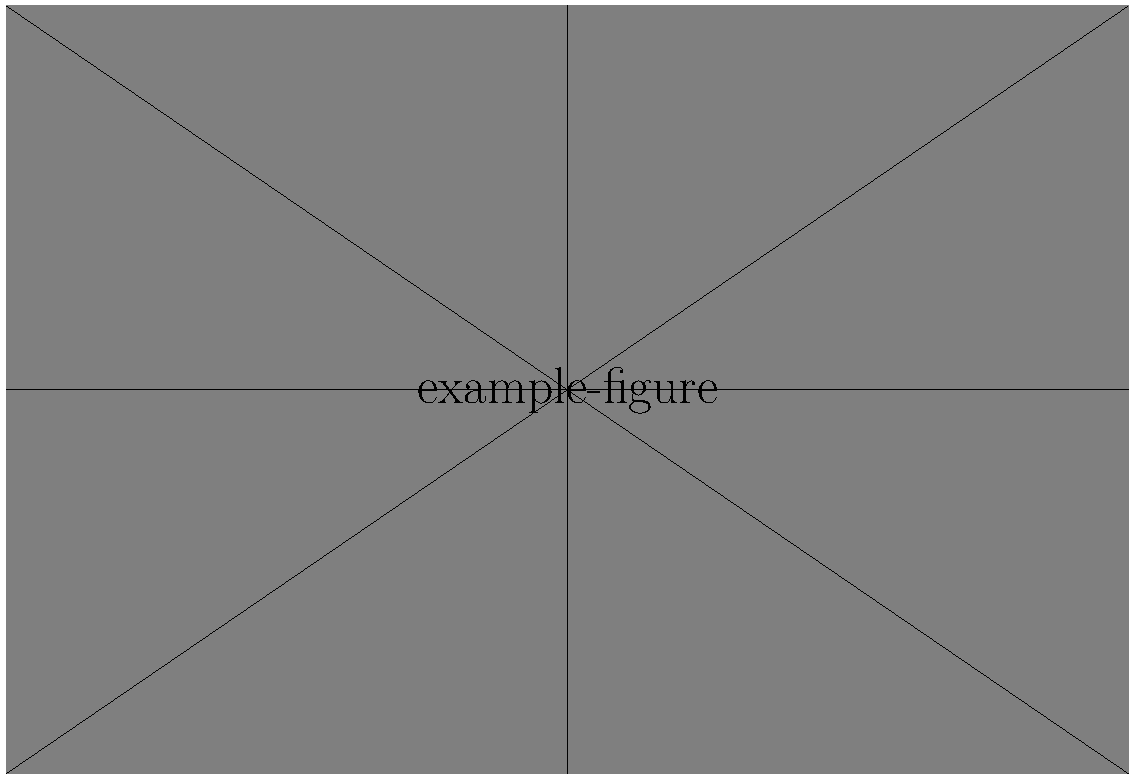
\includegraphics[width=0.8\linewidth]{example-figure}
    \caption{
        一个示例图片,展示了概念图。
    }
    \label{fig:examplefig}
\end{figure}

\subsection{子图}

下面是一个包含 4 个子图的示例(图 \ref{fig:examplesubfigures}),分别为图 \ref{fig:subfigure1}、图 \ref{fig:subfigure2}、图 \ref{fig:subfigure3} 和图 \ref{fig:subfigure4}。

\begin{figure}[htbp]
    \centering
    \subfloat[] {
        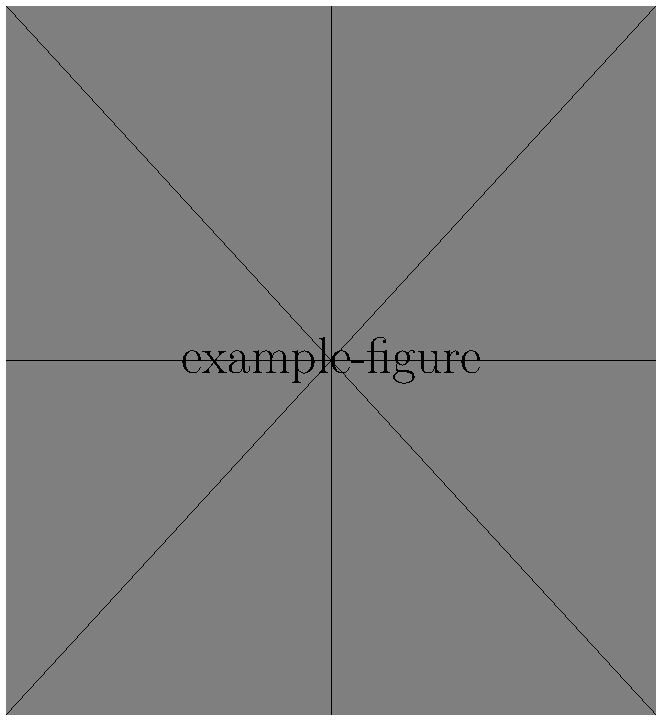
\includegraphics[width=0.31\linewidth]{example-subfigure1}\label{fig:subfigure1}
    }
    \subfloat[] {
        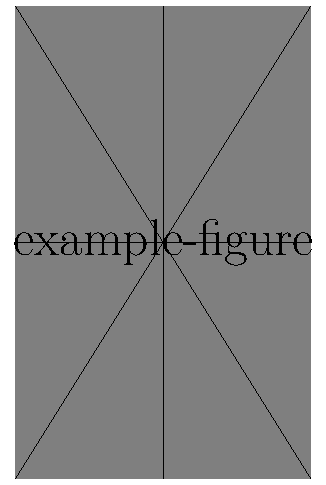
\includegraphics[width=0.23\linewidth]{example-subfigure2}\label{fig:subfigure2}
    }
    \subfloat[] {
        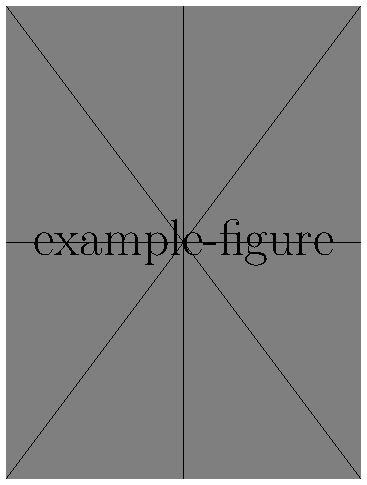
\includegraphics[width=0.24\linewidth]{example-subfigure3}\label{fig:subfigure3}
    }
    \\
    \subfloat[] {
        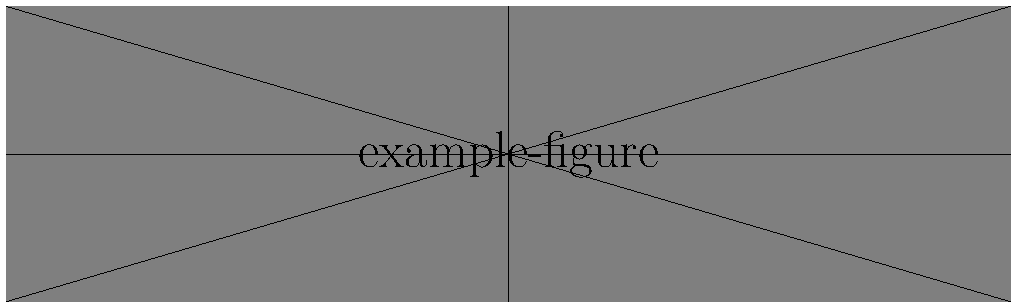
\includegraphics[width=0.8\linewidth]{example-subfigure4}\label{fig:subfigure4}
    }
    \caption{
        示例子图 (a) 子图 1,(b) 子图 2,(c) 子图 3,(d) 子图 4。
    }
    \label{fig:examplesubfigures}
\end{figure}

\section{公式和方程}

此部分包含一个公式的示例。关联矩阵的表达式如公式 \ref{eq:incidence} 所示:

\begin{align}\label{eq:incidence}
    a_{kl}=
    \begin{cases}
        1,  & \text{边 $l$ 离开节点 $k$},\\
        -1, & \text{边 $l$ 进入节点 $k$},\\
        0,  & \text{其他情况},
    \end{cases}
\end{align}
其中 $a_{kl}$ 是关联矩阵的元素,$k$ 是节点编号,$l$ 是边编号。

\section{参考文献}

此部分展示了如何引用参考文献 \cite{article1}。

\bibliographystyle{ieeetr}
\bibliography{../ref}

\end{document}
